\documentclass[12pt]{article}
\usepackage[utf8]{inputenc}
\usepackage{graphicx}
\usepackage{amssymb}
\usepackage{amsthm}
\usepackage{amsmath}
\usepackage{amssymb,mathtools}
\usepackage{lipsum}
\usepackage{array}
\usepackage{wrapfig}
\usepackage{multirow}
\usepackage{tabularx}
\usepackage{graphicx}
\usepackage[percent]{overpic}

\usepackage[a4paper,width=150mm,top=25mm,bottom=25mm,bindingoffset=6mm]{geometry}
\renewcommand{\baselinestretch}{1.2}
\usepackage[style=authoryear,sorting=nty,maxcitenames=1]{biblatex}
\addbibresource{references.bib}

\begin{document}
\begin{titlepage}
	\begin{center}

		\line(1,0){400}\\
		\huge{\bfseries Computational study of far-field acoustic emission by collapsing bubbles}\\
		\line(1,0){400}\\
		[3.5cm]
		{PhD Annual Review Report}\\
		{\today} \\
		[4cm]
		Submitted by\\
		[.5cm]
		{Magu Raam Prasaad R}\\
		[2.cm]
		Department of Mechanical Engineering\\
		Indian Institute of Science\\
		Bangalore

	\end{center}
\end{titlepage}
\section{Introduction}
The high-speed rotary motion of submerged propeller blades results in the formation of cavitation bubbles. These cavitation bubbles undergo significant shape variations and collapse violently. Cloud of collapsing cavitation bubbles emits blastwaves and are the source of acoustic waves.
Accurate prediction of the sound waves emitted from interacting collapsing bubbles is of significant importance in marine hydrodynamics.
The present work aims to carry out a large-scale numerical simulation of single and multiple cavitation bubble collapse process to develop a detailed understanding of the acoustic wave emission and propagation.

Early investigations on the acoustic waves emitted from oscillating bubbles relied on theoretical analysis of the simplified radial dynamics (\cite{Rayleigh},\cite{Plesset}, \cite{Prosperetti}). Developments in computational power and methodologies (\cite{SHUKLA20107411}, \cite{SHUKLA2014508}, \cite{Pantano}) has enabled detailed numerical simulation of the aspherical collapse process (\cite{freund2009shock}, \cite{jamaluddin}). However,
numerical simulation of acoustic waves emitted by a cloud of bubbles is computationally expensive. To overcome the challenge, we use the massively parallel high-speed compressible multiphase solver developed in the lab. We use the higher-order low dissipative (WENO-ADER) scheme with interface and shock-capturing to solve the axisymmetric bubble collapse problem. We use the Kirchhoff integral solver to compute the far-field acoustic pressure. In this work, we have studied the error convergence of numerical integration of the Kirchhoff formula and computed the acoustic pressure emitted by an axisymmetric bubble collapse. 

\section{Mathematical formulation}
\subsection{Kirchhoff integral formula}
\begin{figure}[h!]\label{Kirchhoff}
	\centering
	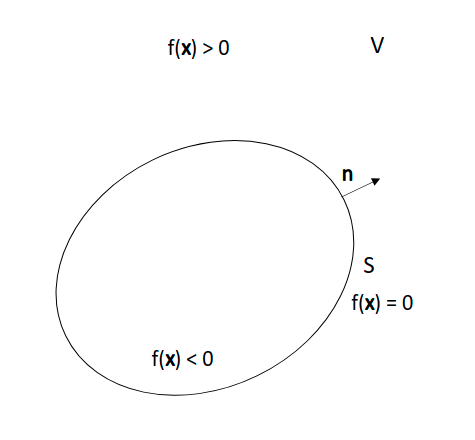
\includegraphics[width=60mm]{images/kirchhoff_surface.png}
	\caption{Stationary Kirchhoff surface $S$ encloses sound source}
\end{figure}
In this section, we derive the Kirchhoff formula for a stationary control surface (\cite{FARASSAT1988451}). We chose a control surface $S$ that encloses all the acoustic sources (\ref{Kirchhoff}), and the pressure perturbations $p$ satisfies the homogeneous wave equation
\begin{equation}\label{Wave equation}
	\Bigg( \frac{1}{c_{0}^2}\frac{\partial{}^{2}}{\partial{t}^{2}}- \nabla{}^{2} \Bigg) p = 0 \quad \quad \textrm{in} \ V.
\end{equation}
The control surface S is defined by $f(\mathbf{x}) = 0$, $f(\mathbf{x}) > 0$ for $\mathbf{x}$ in V and $f(\mathbf{x}) < 0$ for $\mathbf{x}$ inside surface S. We scale the function $f$ such that $\nabla f = \mathbf{n}$. Then the Heaviside function of $f(\mathbf{x})$    is
\begin{equation}\label{Heaviside}
	H(f) =\begin{cases}
		1, & \text{for $\mathbf{x}$ in V}.     \\
		0, & \text{for $\mathbf{x}$ inside S}.
	\end{cases}
\end{equation}
The gradient of the Heaviside function is given by
\begin{equation}\label{Gradient Heaviside}
	\nabla H(f) = \delta (f) \mathbf{n}.
\end{equation}
We define the pressure $p$ as a generalized function $pH(f)$ (\cite{ffowcs1969sound}) where
\begin{equation}\label{Generalized_Functions}
	p H(f) =\begin{cases}
		p , & \text{for $\mathbf{x}$ in V}.     \\
		0,  & \text{for $\mathbf{x}$ inside S}.
	\end{cases}
\end{equation}
The generalized pressure $pH(f)$ is defined everywhere in space, unlike $p$ defined only in $V$. We will derive the acoustic wave equation for the generalised pressure. Using (\ref{Gradient Heaviside}), the gradient of $pH$ is
\begin{equation}
	\nabla (pH) = \nabla p H + p \delta(f)\mathbf{n}.
\end{equation}
Therefor the Laplacian is given by
\begin{equation}\label{Laplacian}
	\nabla^2 (pH) = \nabla^2 p H +  \frac{\partial p}{\partial n}\delta(f) + \nabla.(p \delta(f)\mathbf{n}).
\end{equation}
The partial derivative in time is
\begin{equation}\label{Time derivative}
	\frac{\partial^2}{\partial t^2}(pH) = \frac{\partial^2 p }{\partial t^2}H.
\end{equation}
We premultiply (\ref{Time derivative}) with $1/{c_{0}^2}$ and subtract (\ref{Laplacian}) to obtain the acoustic wave equation in generalised pressure
\begin{equation}
	\Bigg( \frac{1}{c_{0}^2}\frac{\partial{}^{2}}{\partial{t}^{2}}- \nabla{}^{2} \Bigg) pH = H\Bigg( \frac{1}{c_{0}^2}\frac{\partial{}^{2}}{\partial{t}^{2}}- \nabla{}^{2} \Bigg) p - \frac{\partial p}{\partial n}\delta(f) - \nabla.(p \delta(f)\mathbf{n}),
\end{equation}
or
\begin{equation}\label{Generalized Wave Equation}
	\Bigg( \frac{1}{c_{0}^2}\frac{\partial{}^{2}}{\partial{t}^{2}}- \nabla{}^{2} \Bigg) pH = -\frac{\partial p}{\partial n}\delta(f) - \nabla.(p \mathbf{n} \delta(f)).
\end{equation}
The right side of the equation (\ref{Generalized Wave Equation}) is non-zero only at surface $S$, as it contains $\delta (f)$. The acoustic wave equation (\ref{Generalized Wave Equation}) in generalized variables is valid in the entire unbounded space. Therefore we can use free-space Green's function to solve the equation. The Green's function is the solution of wave equation for an impulsive point source $\delta(\mathbf{x} - \mathbf{y})\delta(t - \tau)$ placed at point $\mathbf{y}$ and time $\tau$
\begin{equation}\label{green}
	\Bigg( \frac{1}{c_{0}^2}\frac{\partial{}^{2}}{\partial{t}^{2}}- \nabla{}^{2} \Bigg){G(\mathbf{x}, t; \mathbf{y}, \tau )} = \delta{(\mathbf{x} - \mathbf{y})}\delta{(t - \tau)}.
\end{equation}
The Green's function for the acoustic wave operator (\cite{howe2003theory}) in three dimensions is
\begin{equation}\label{Green's Function}
	G(\mathbf{x}, t; \mathbf{y}, \tau ) = \frac{\delta \Big(t - \tau - \frac{|\mathbf{x} - \mathbf{y}|}{c_{0}}\Big)}{4\pi|\mathbf{x} - \mathbf{y}|}.
\end{equation}
The solution for arbirtary source can be obtained by multiplying $s(\mathbf{y}, \tau)$ in (\ref{green})
\begin{equation}
	\Bigg( \frac{1}{c_{0}^2}\frac{\partial{}^{2}}{\partial{t}^{2}}- \nabla{}^{2} \Bigg)s(\mathbf{y}, \tau){G(\mathbf{x}, t; \mathbf{y}, \tau )} = s(\mathbf{y}, \tau)\delta{(\mathbf{x} - \mathbf{y})}\delta{(t - \tau)},
\end{equation}
Integrating both sides
\begin{equation}
	\Bigg( \frac{1}{c_{0}^2}\frac{\partial{}^{2}}{\partial{t}^{2}}- \nabla{}^{2} \Bigg) \int s(\mathbf{y}, \tau){G(\mathbf{x}, t; \mathbf{y}, \tau )} d\mathbf{y}d\tau  = \int s(\mathbf{y}, \tau)\delta{(\mathbf{x} - \mathbf{y})}\delta{(t - \tau)} d\mathbf{y}d\tau,
\end{equation}
and using the properties of delta function, we get the solution for the acoustic wave equation with source $s(\mathbf{x}, t)$
\begin{equation}
	\Bigg( \frac{1}{c_{0}^2}\frac{\partial{}^{2}}{\partial{t}^{2}}- \nabla{}^{2} \Bigg) p(\mathbf{x}, t)  = s(\mathbf{x}, t),
\end{equation}
where,
\begin{equation}\label{pressure}
	p(\mathbf{x}, t) = \int s(\mathbf{y}, \tau){G(\mathbf{x}, t; \mathbf{y}, \tau )} d\mathbf{y}d\tau.
\end{equation}
We can use the above relation to solve the acoustic wave equation (\ref{Generalized Wave Equation})
\begin{equation}
	\begin{split}
		(pH)(\mathbf{x}, t) = &-\frac{1}{4\pi}\int {\frac{\partial p}{\partial n}\delta(f) \frac{\delta \Big(t - \tau - \frac{|\mathbf{x} - \mathbf{y}|}{c_{0}}\Big)}{|\mathbf{x} - \mathbf{y}|}} d\mathbf{y}d\tau \\
		&-\frac{1}{4\pi}\int \nabla_{\mathbf{y}}.(p \mathbf{n} \delta(f)){\frac{\delta \Big(t - \tau - \frac{|\mathbf{x} - \mathbf{y}|}{c_{0}}\Big)}{|\mathbf{x} - \mathbf{y}|}} d\mathbf{y}d\tau.
	\end{split}
\end{equation}
\begin{equation}
	\begin{split}
		(pH)(\mathbf{x}, t) = &-\frac{1}{4\pi}\int {\frac{\partial p}{\partial n}\delta(f) \frac{\delta \Big(t - \tau - \frac{|\mathbf{x} - \mathbf{y}|}{c_{0}}\Big)}{|\mathbf{x} - \mathbf{y}|}} d\mathbf{y}d\tau \\
		&-\frac{1}{4\pi}\nabla_{\mathbf{x}}.\int (p \mathbf{n} \delta(f)){\frac{\delta \Big(t - \tau - \frac{|\mathbf{x} - \mathbf{y}|}{c_{0}}\Big)}{|\mathbf{x} - \mathbf{y}|}} d\mathbf{y}d\tau.
	\end{split}
\end{equation}
We use the following property to convert volume integral to surface integral (\cite{FARASSAT1988451}).
\begin{equation}\label{volume surface}
	\int \phi (\mathbf{y}) \delta (f) \mathbf{n} d\mathbf{y} = \int_{S} \phi (\mathbf{y}) \mathbf{n} dS
\end{equation}
We use the above property to convert volume integral to surface integral on $S$
\begin{equation}
	\begin{split}
		(pH)(\mathbf{x}, t) = &-\frac{1}{4\pi}\int {\frac{\partial p}{\partial n} \frac{\delta \Big(t - \tau - \frac{|\mathbf{x} - \mathbf{y}|}{c_{0}}\Big)}{|\mathbf{x} - \mathbf{y}|}} dSd\tau \\
		&-\frac{1}{4\pi}\nabla_{\mathbf{x}}.\int (p \mathbf{n} ){\frac{\delta \Big(t - \tau - \frac{|\mathbf{x} - \mathbf{y}|}{c_{0}}\Big)}{|\mathbf{x} - \mathbf{y}|}} dSd\tau.
	\end{split}
\end{equation}
Using the property of delta function we obtain
\begin{equation}
	\begin{split}
		(pH)(\mathbf{x}, t) = &-\frac{1}{4\pi}\int_{S} { \Big[\frac{\partial p}{\partial n}\Big] \frac{dS}{|\mathbf{x} - \mathbf{y}|}}  \\
		&-\frac{1}{4\pi}\nabla_{\mathbf{x}}.\int_{S} [p]\mathbf{n}{\frac{dS}{|\mathbf{x} - \mathbf{y}|}} .
	\end{split}
\end{equation}
The square bracket implies the functions are computed at the retarded time i.e, $[p] = p(\mathbf{y}, t - \frac{|\mathbf{x} - \mathbf{y}|}{c})$. Simplifying the equation further, we obtain the Kirchhoff formula for a stationary control surface (\cite{FARASSAT1988451}, \cite{jamaluddin}).
\begin{equation}\label{Kirchhoff Integral}
	\begin{split}
		(pH)(\mathbf{x}, t) = -\frac{1}{4\pi}\int_{S}\Big[  \frac{p}{r^{2}}\frac{\partial r}{\partial n} - \frac{1}{r}\frac{\partial p}{\partial n} + \frac{1}{c r}\frac{\partial r}{\partial n}\frac{\partial p}{\partial \tau} \Big]_{\tau} dS.
	\end{split}
\end{equation}
Where, $r = |\mathbf{x} - \mathbf{y}|$, the square bracket again implies the functions are computed at the retarded time $\tau = t - r/c$.
\subsection{Numerical integration}
\begin{figure}[h!]
	\centering
	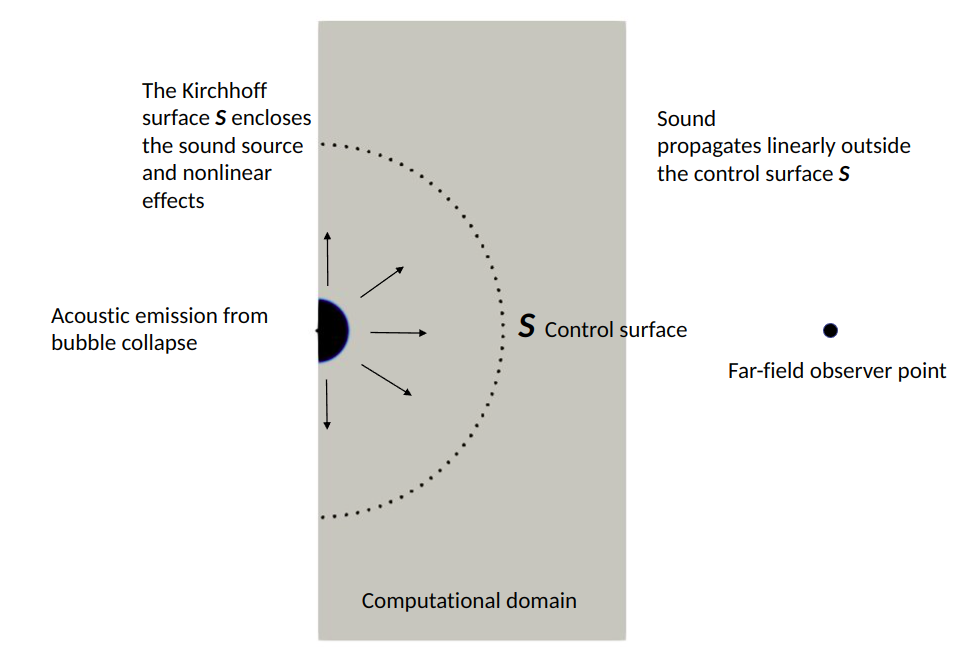
\includegraphics[scale=0.3]{images/schematic.png}
	\caption{Schematic of far-field acoustic data computed from CFD solver using the Kirchhoff integral method.}
	\label{schematic}
\end{figure}
In this work, we compute the sound wave emitted by an axisymmetric bubble collapse at the far field. The schematic \ref{schematic} shows the axisymmetric domain and the Kirchhoff control surface. We discretize the circular arc with quadrature points, and the pressure data is interpolated from cell centers to quadrature points using the fourth-order WENO polynomial. The pressure is interpolated at emission time using the four-point Lagrange polynomial. The pressure data on the circular arc is revolved around the axis to create a spherical surface of quadrature points. Now we can use the Kirchhoff integral formula derived in the previous section for the spherical surface to compute the acoustic pressure at the far field. We use the spherical coordinates and rewrite the integral as,
\begin{equation}
	\begin{split}
		p'(r, \theta, \phi,t) =  \frac{1}{4\pi}\int_{0}^{2\pi}\int_{0}^{\pi}\Big[  \frac{p'}{r'^{2}}&\frac{\partial r'}{\partial n} - \frac{1}{r'}\frac{\partial p'}{\partial n} + \frac{1}{c r'}\frac{\partial r'}{\partial n}\frac{\partial p'}{\partial \tau} \Big]_{\tau} R^2\sin\theta d\theta d \phi.  
	\end{split} 
\end{equation}
The above integral is numerically computed using the mid-point rule 
\begin{equation}
	\begin{split}
		p'(r, \theta, \phi,t) =  \frac{1}{4\pi} \sum_{i}^{N_{\theta}}\sum_{j}^{N_{\phi}}  \Big[  \frac{p'}{r'^{2}}&\frac{\partial r'}{\partial n} - \frac{1}{r'}\frac{\partial p'}{\partial n} + \frac{1}{c r'}\frac{\partial r'}{\partial n}\frac{\partial p'}{\partial \tau} \Big]_{\tau} R^2\sin\theta \Big|_{i, j} \Delta \theta \Delta \phi.  
	\end{split} 
\end{equation}

\section{Results}
\subsection{Convergence of Kirchhoff integral}
\begin{figure}[h!]
	\centering
	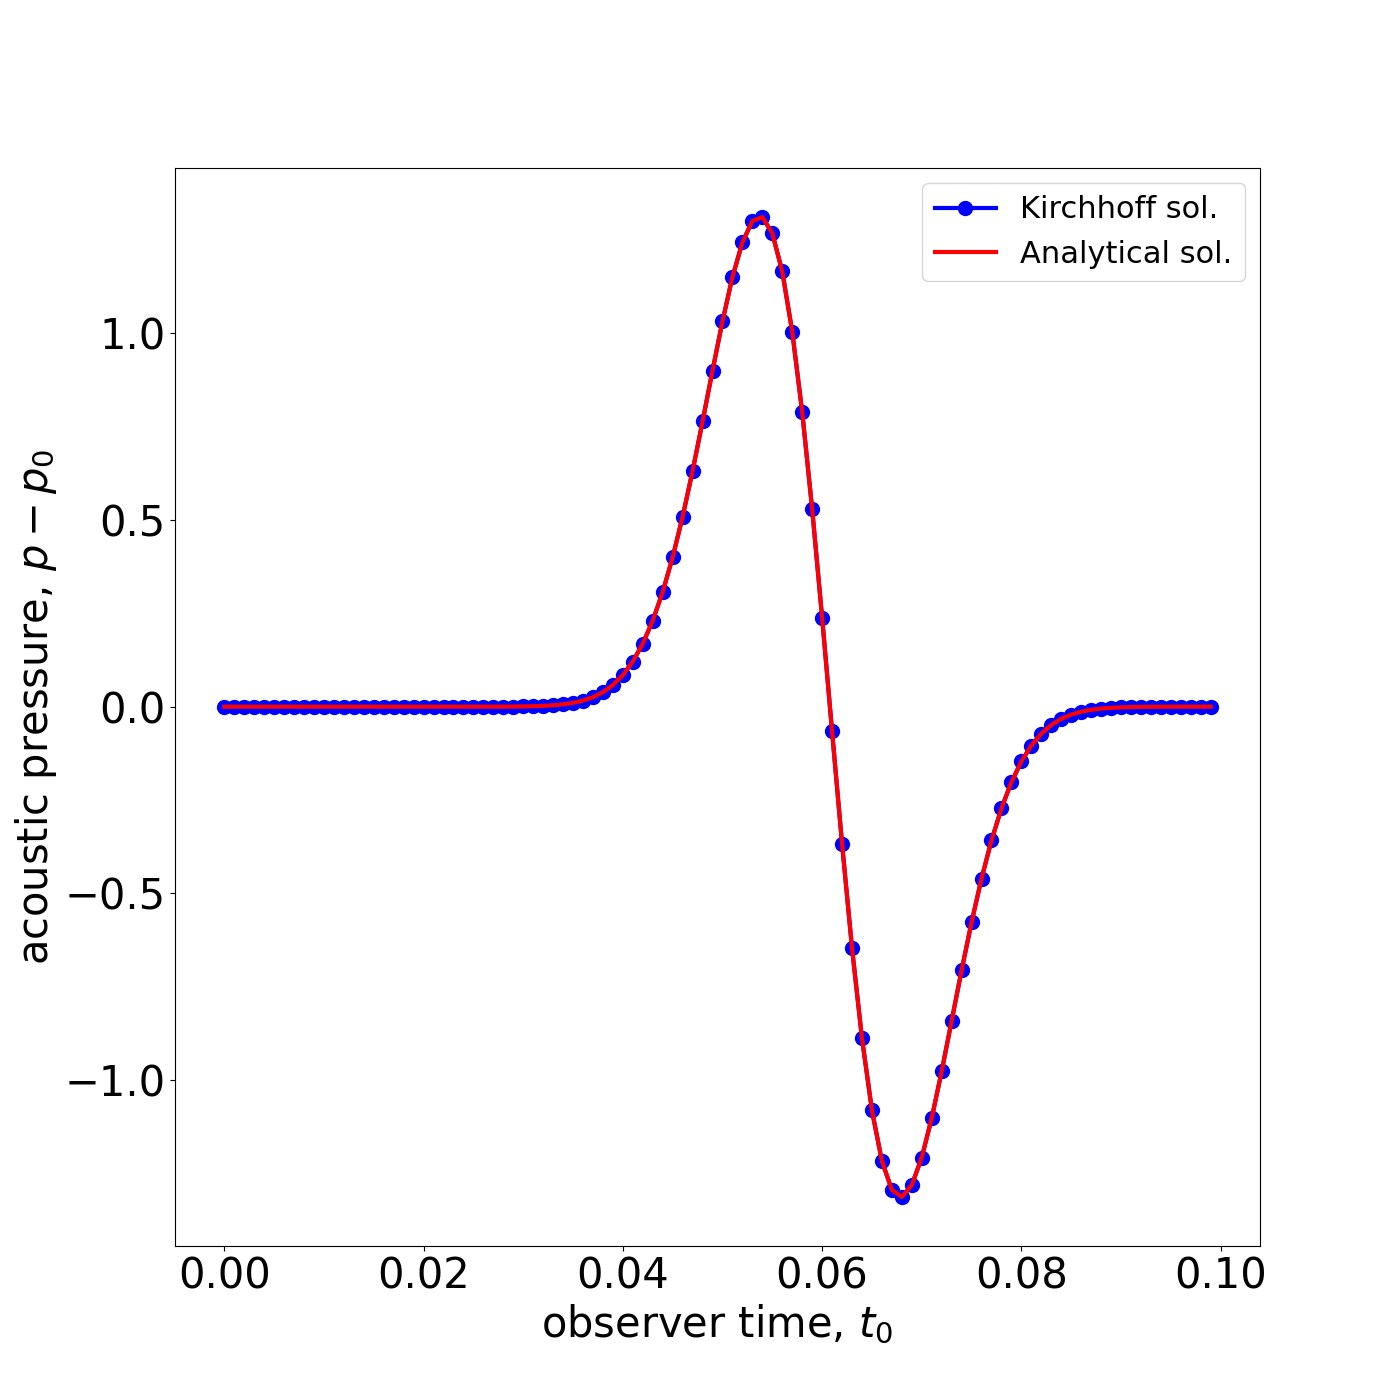
\includegraphics[scale=0.3]{images/Pressure.png}
	\caption{Acoustic pressure computed using the Kirchhoff method and compared with the analytical solution at observer point $(x, y, z) = (3.0, 3.0, 3.0).$}
	\label{comparison}
\end{figure}
\begin{figure}[h!]
	\centering
	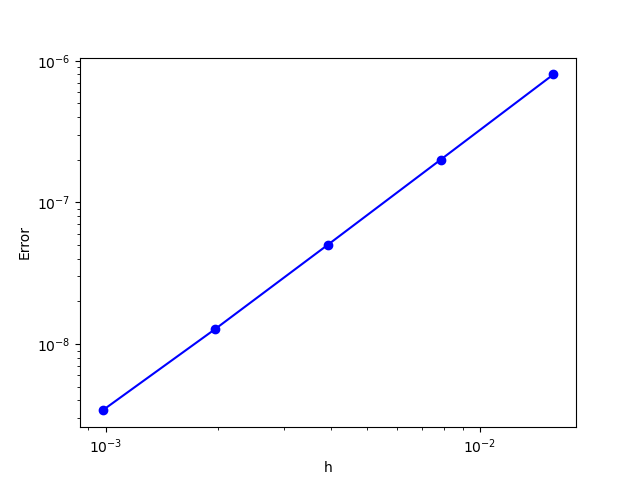
\includegraphics[scale=0.6]{images/convergence.png}
	\caption{We have obtained second-order convergence for the Kirchhoff integral computed using the mid-point rule.}
	\label{convergence}
\end{figure}
We compute the Kirchhoff integral for the pressure emitted by a monopole source
$p'(\mathbf{x}, t) = -\frac{1}{4\pi} \frac{  q(t - \frac{r}{c_{0}}) }{r}$. We choose a monopole of strength $q(t) = 2(t - t0)f_{0}^{2}\exp( -f_{0}^2(t - t_{0})^{2})$,
where $f_{0} = 100$ is the dominant frequency and $t_{0} = \frac{4}{f_{0}}$. Acoustic pressure is computed at observer point ($x_{0}, y_{0}, z_{0}$) $= (3.0, 3.0, 3.0)$ using the Kirchhoff method and compared with the analytical solution as shown in figure \ref{comparison}. We chose a sphere of radius $R = 1.0$. We obtain second-order convergence of error for the numerical integration as shown in figure \ref{convergence}.
\subsection{Rayleigh collapse of bubble}
\begin{figure}[h!]
	\centering
	\begin{overpic}[scale=0.5]{images/initial_condition.png}
	\end{overpic}
	\caption{Initial condition}
	\label{Initial condition}
\end{figure}
\begin{figure}[h!]
	\centering
	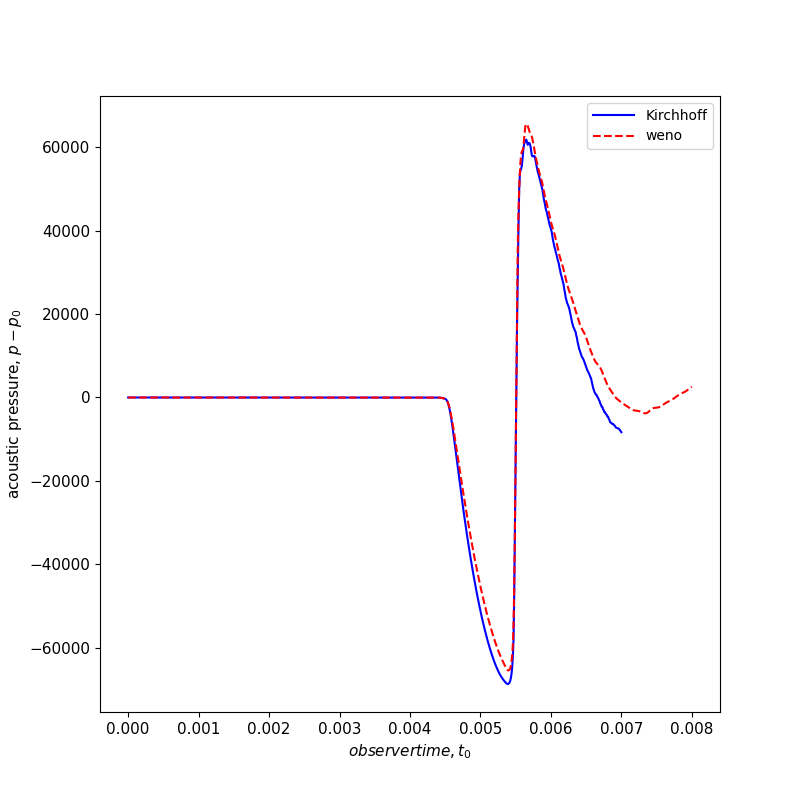
\includegraphics[scale=0.6]{images/structured_pressure.png}
	\caption{Comparison of acoustic pressure at observer point from flow solver and Kirchhoff solver.}
	\label{comparison}
\end{figure}
In this section, we compute sound waves emitted by the collapse of an air bubble placed in a water medium. We assume an axisymmetric bubble collapse and solve the compressible multiphase Euler equations.
We choose an axisymmetric domain $\Omega = [-10R,10R]\times[0,10R]$ and a bubble of radius $R = 38 mm$ is placed at origin. The domain is discretized into $500\times 250$ cells. The initial conditions for air bubble and water medium are set as shown in figure \refeq{Initial condition}. The radius of the spherical Kirchhoff surface is $6R$ and the far-field observer point is at $(0, 9R)$. The number of quadrature points along $\theta$ and $\phi$ directions are $N_{\theta} = 500$ and $N_{\phi} = 1000$. The speed of sound in the far-field acoustic medium is obtained from $\sqrt{\gamma(P + P_{\infty})/\rho}$. The comparison of acoustic pressure at observer point from flow solver and Kirchhoff solver is shown in figure \ref{comparison}.


\section{Conclusion and future work}
We have shown the second-order convergence for the numerical integration of the Kirchhoff integral using the mid-point rule for the acoustic waves emitted by the monopole. We have to implement the fourth-order accurate axi-symmetric Kirchhoff solver. And compute far-field sound waves emitted by single and multiple bubble collapse process.

\printbibliography
\end{document}

